\documentclass[a4paper,12pt]{article} % тип документа

%  Русский язык
\usepackage[T2A]{fontenc}			% кодировка
\usepackage[utf8]{inputenc}			% кодировка исходного текста
\usepackage[english,russian]{babel}	% локализация и переносы

\usepackage{graphicx, scalerel}               % импорт изображений
\usepackage{wrapfig}                % обтекаемые изображения
\graphicspath{{pictures/}}          % обращение к подкаталогу с изображениями
\usepackage[14pt]{extsizes}         % для того чтобы задать нестандартный 14-ый размер шрифта
\usepackage[warn]{mathtext}         % русский язык в формулах
\usepackage{indentfirst}            % indent first
\usepackage[margin = 25mm]{geometry}% отступы полей
\usepackage[table,xcdraw]{xcolor}   % таблицы
\usepackage{amsmath,amsfonts,amssymb,amsthm,mathtools} % Математика
\usepackage{wasysym}                % ???
\usepackage{upgreek}                % ???  
\usepackage{caption}
\usepackage{multirow}
\captionsetup{labelsep=period}
\usepackage[font=small,labelfont=bf]{caption}
\usepackage{gensymb} % degree symbol
\usepackage{tikz}
\usetikzlibrary{positioning}


\begin{document}
	
	
	\begin{center}
		
		\textbf{НАЦИОНАЛЬНЫЙ ИССЛЕДОВАТЕЛЬСКИЙ УНИВЕРСИТЕТ \\ <<МОСКОВСКИЙ ФИЗИКО-ТЕХНИЧЕСКИЙ ИНСТИТУТ>>}
		\vspace{13ex}
		
		\textbf{Лабораторная работа 5.2.1\\ <<Опыт Франка-Герца>>}
		\vspace{40ex}
		
		\normalsize{Шумаков Иван Игоревич \\ студент группы Б01-009\\ 3 курс ФРКТ\\}
	\end{center}
	
	\vfill 
	
	\begin{center}
		г. Долгопрудный\\ 
		2022 г.
	\end{center}
	
	
	\thispagestyle{empty} % выключаем отображение номера для этой страницы
	\newpage

	\textbf{Цель работы:} Методом электронного возбуждения измерить энергию первого уровня атома гелия в динамическом и статическом режимах.\par
	\textbf{В работе используются:} Трёхэлектродная лампа ЛМ-2, батарея 4,5 В, микроамперметр, понижающий трансформатор, осциллограф, блок источников питания, вольтметр В7-22А\par
		
	\section{Теоретические положения}

		Опыт Франка-Герца подтверждает существование дискретных уровней энергии атомов. Разреженный одноатомный газ заполняет трёхэлектродную лампу. Электроны, испускаемые разогретым катодом, ускоряются в постоянном электрическом поле, созданном между катодом и сетчатым анодом лампы. Передвигаясь от катода к аноду, электроны сталкиваются с атомами гелия.
		\begin{itemize}
			\item энергия электрона недостаточна, чтобы возбудить/ионизировать атом -> \textit{упругое столкновение}, электрон не теряет энергию
			\item при большой разности потенциалов энергия электрона достаточна для возбуждения атомов -> \textit{неупругое столкновение}, кинетическая энергия передаётся одному из атомных электронов, в результате чего происходит:
			\begin{itemize}
				\item \textbf{возбуждение} - переход одного из атомных электронов на свободный энергетический уровень
				\item \textbf{ионизация} - отрыв электрона от атома 
			\end{itemize}
		\end{itemize}

		\begin{figure}[h]
			\begin{center}
				\begin{minipage}[h]{0.45\linewidth}
					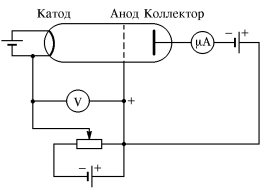
\includegraphics[width=1\linewidth]{img/fig1.png}
					\caption{Схема опыта Франка и Герца} %% подпись к рисунку
					\label{ris:experimoriginal} %% метка рисунка для ссылки на него
				\end{minipage}
				\hfill 
					\begin{minipage}[h]{0.45\linewidth}
					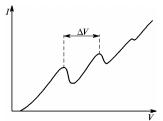
\includegraphics[width=1\linewidth]{img/fig2.png}
					\caption{Схематический вид зависимости тока коллектора от напряжения на аноде}
					\label{ris:experimcoded}
					\end{minipage}
			\end{center}
		\end{figure}

		Объясним вид зависимости тока коллектора (измеряется микроамперметром) от напряжения на аноде. 
		При увеличении потенциала анода ток в лампе сначала растёт (зависимость, подобная ВАХ вакуумного диода). 
		Когда энергия электронов становится достаточной для возбуждения атомов, ток коллектора резко уменьшается. 
		Это происходит потому, что при неупругих соударениях с атомами электроны теряют свою энергию и не могут преодолеть задерживающее напряжение (около 1 В) между анодом и коллектором. 
		При дальнейшем увеличении потенциала ток коллектора вновь возрастает: электроны, испытавшие неупругие соударения, при дальнейшем движении к аноду успевают набрать энергию, достаточную для преодоления задерживающего потенциала. 
		Следующее замедление роста тока происходит в момент, когда часть электронов неупруго сталкивается с атомами два раза. 
		Таким образом, на кривой зависимости тока коллектора от напряжения анода имеется ряд максимумов и минимумов, отстоящих друг от друга на равные расстояния, равные энергии первого возбуждённого состояния.

	\section{Ход работы}

		\subsection{Динамический метод}

			В данном опыте были получены осциллограммы, характеризующие изменение тока коллектора от напряжения на аноде.\par
			\begin{figure}[h!]
                \centering
                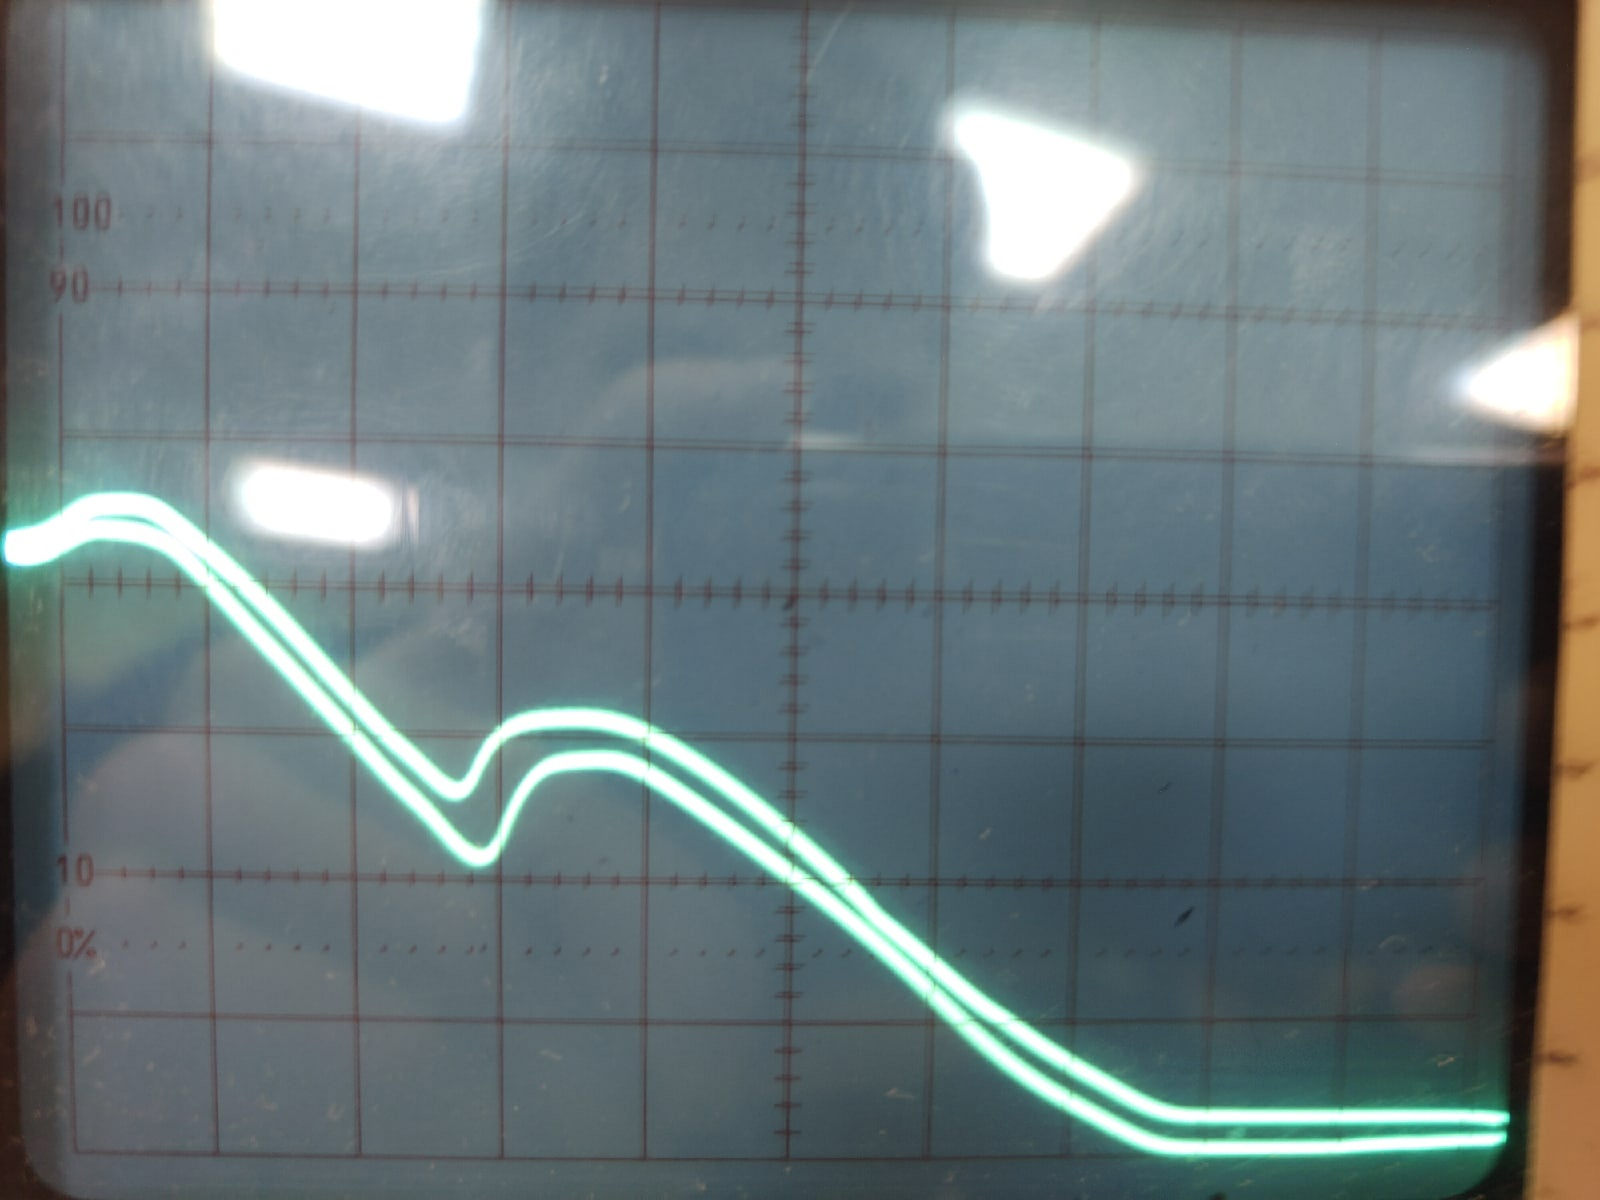
\includegraphics[width=10cm]{img/din1.jpg}
                \caption{осциллограмма при 4В}
                \label{din1}
            \end{figure}\par
	\newpage
			\begin{figure}[h!]
                \centering
                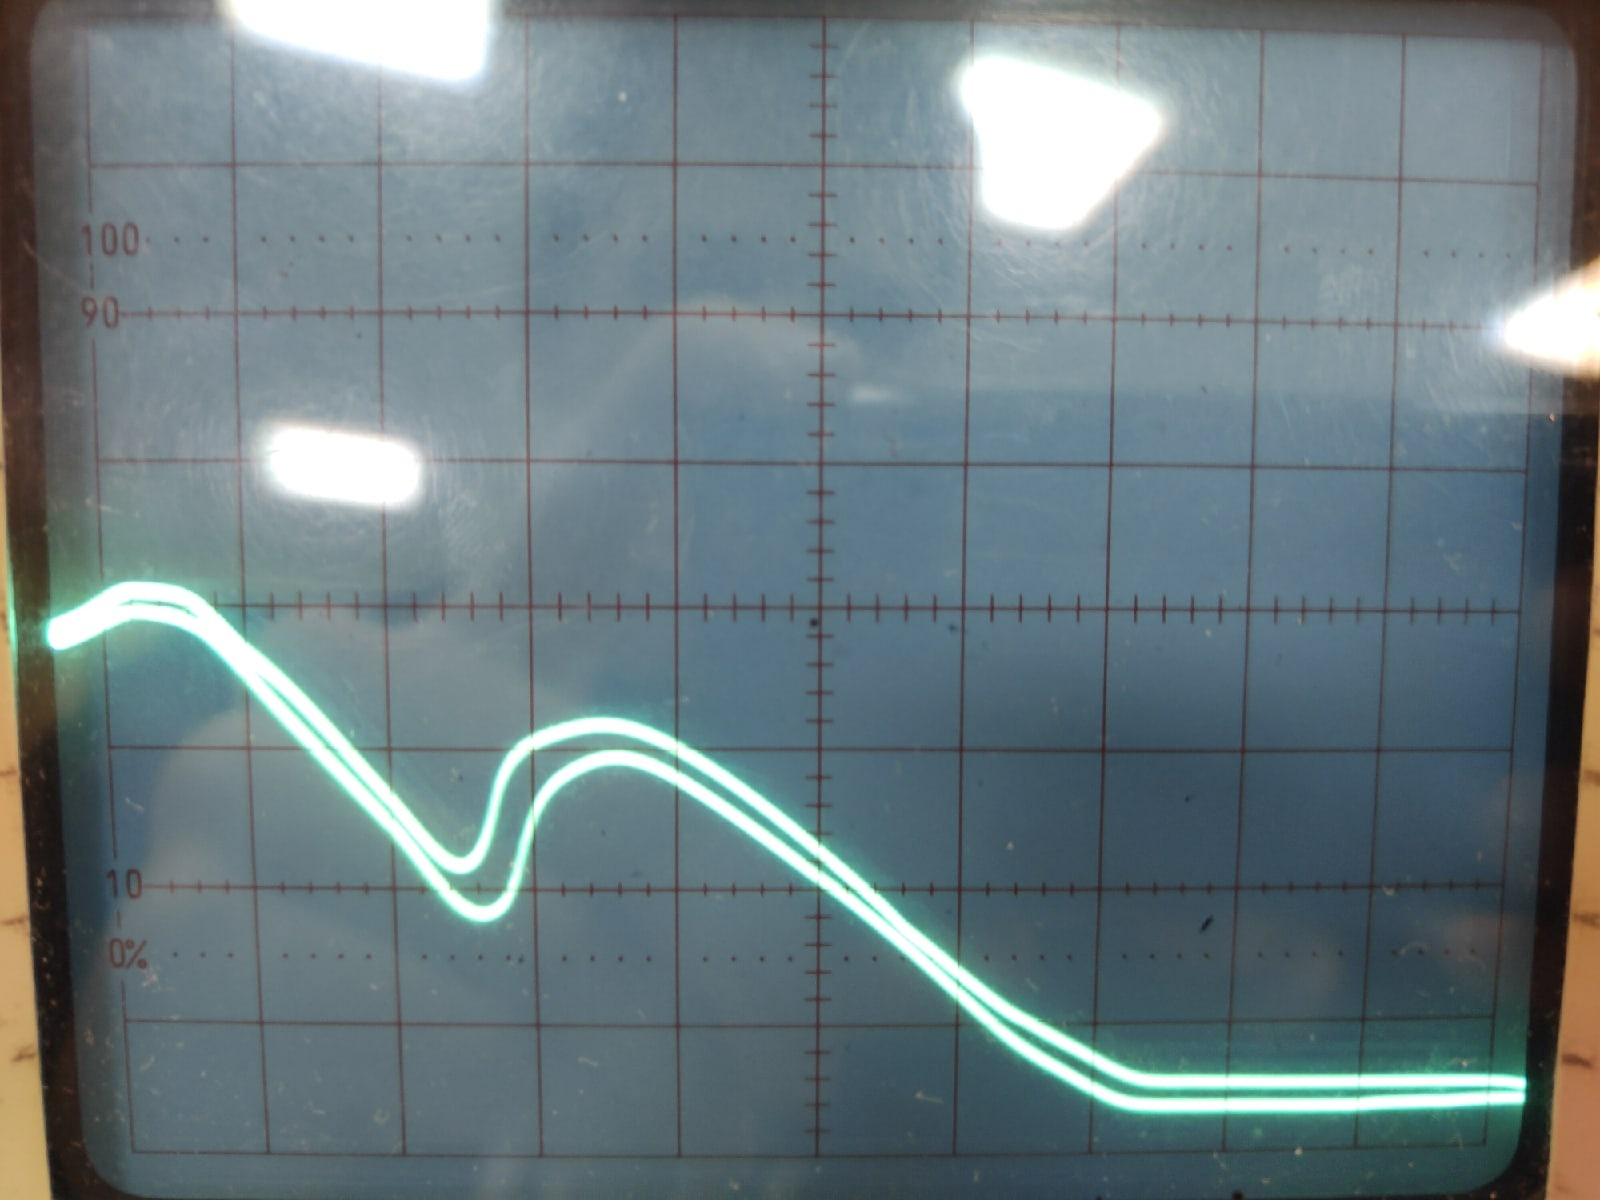
\includegraphics[width=10cm]{img/din2.jpg}
                \caption{осциллограмма при 6В}
                \label{din2}
            \end{figure}\par
			\begin{figure}[h!]
                \centering
                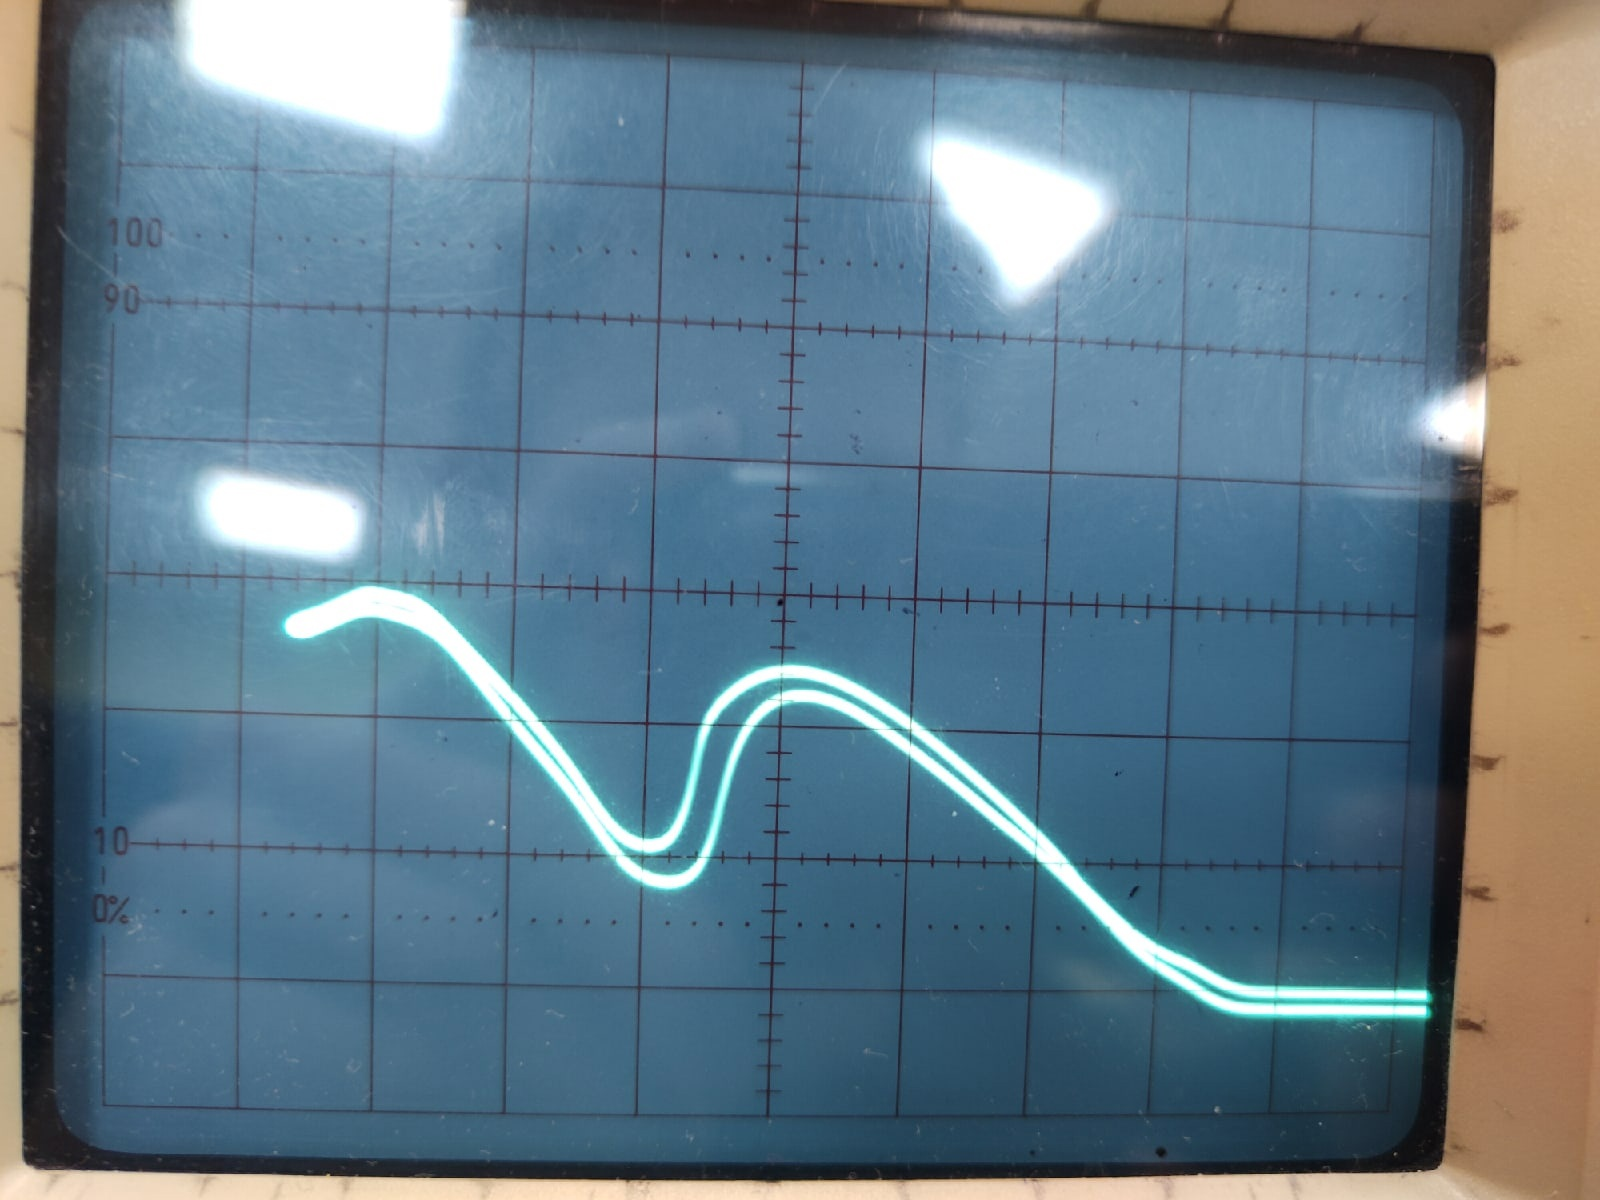
\includegraphics[width=10cm]{img/din3.jpg}
                \caption{осциллограмма при 9В}
                \label{din3}
            \end{figure}\par
			По графикам были определены расстояния между максимумами:
			\begin{table}[h!]
				\centering
				\begin{tabular}{|c|c|}
				\hline
				$U_\text{коллектор}$ [B] & $\Delta U_\text{максимумы}$ [B]      \\ \hline
				4                        & 16                                   \\ \hline
				6                        & 16                                   \\ \hline
				9                        & 15                                   \\ \hline
				\end{tabular}
			\end{table}
			Погрешность определения расстояний между максимумами равна:
			\begin{equation}
				\Delta = 1 [B] \hspace{10mm}
				\delta = 0.07
			\end{equation}
			Таким образом энергия первого уровня атома гелия равна:
			\begin{equation}
				E_H = (16 \pm 1) [\text{эВ}]
			\end{equation}

		\subsection{Статический метод}
				
			В данном опыте были измерены значения тока коллектора и разности потенциалов в камере.
			По этим данным были построены графики и по ним получены расстояния между экстремумами.\par
			Получившыеся графики:
			\begin{figure}[h!]
                \centering
                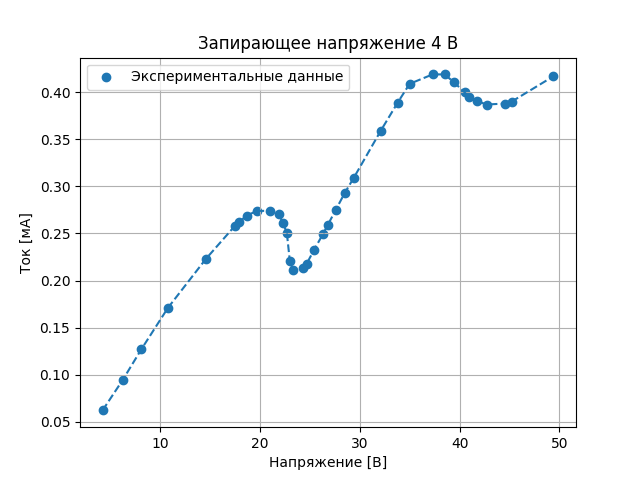
\includegraphics[width=7cm]{img/gra1.png}
                \caption{Зависмость при 4В}
                \label{gra1}
            \end{figure}\par
			\begin{figure}[h!]
                \centering
                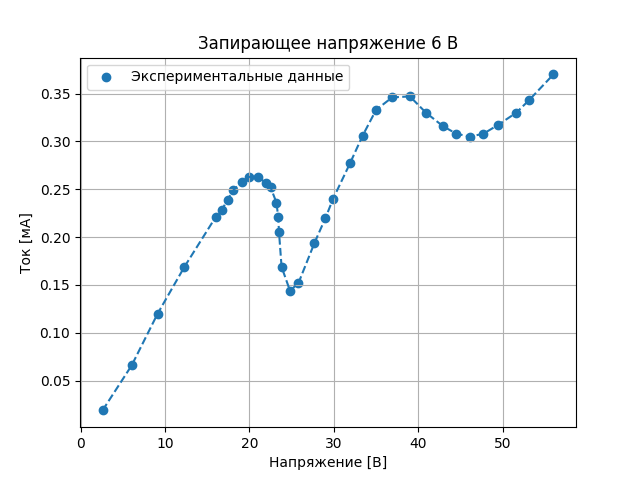
\includegraphics[width=7cm]{img/gra2.png}
                \caption{Зависмость при 6В}
                \label{gra1}
            \end{figure}\par
			\begin{figure}[h!]
                \centering
                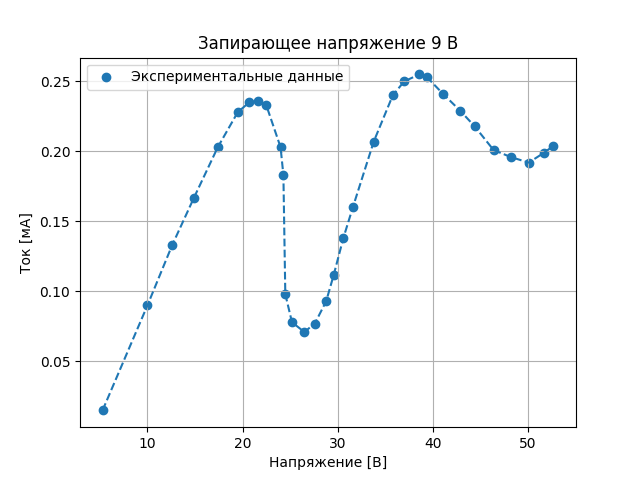
\includegraphics[width=7cm]{img/gra3.png}
                \caption{Зависмость при 9В}
                \label{gra1}
            \end{figure}\par
	\newpage
			Расстояние между максимумами и минимумами:
			\begin{table}[h!]
				\centering
				\begin{tabular}{|c|c|c|}
				\hline
				$U_\text{коллектор}$ [B] & $\Delta U_\text{максимумы}$ [B]  & $\Delta U_\text{минимумы}$ [B]\\ \hline
				4                        & 17                           	& 23.6                      	\\ \hline
				6                        & 18.5                         	& 21.3                      	\\ \hline
				9                        & 17.4                         	& 19.4                      	\\ \hline
				\end{tabular}
			\end{table}\par
			По полученным данным можно оценить энергию возбуждения первого уровня атома гелия:
			\begin{equation}
				E \approx (17.5 \pm 1) [\text{эВ}] 
			\end{equation}
			
	\newpage
			Экспериментальные данные:\par	
			\begin{table}[h!]
				\centering
				\begin{tabular}{cclcclcc}
				\multicolumn{1}{r}{4В}                   & \multicolumn{1}{l}{}       &                       & \multicolumn{1}{l}{6В}          & \multicolumn{1}{l}{}       &                       & \multicolumn{1}{l}{9В}          & \multicolumn{1}{l}{}       \\ \cline{1-2} \cline{4-5} \cline{7-8} 
				\multicolumn{1}{|c|}{$U [B]$} 			 & \multicolumn{1}{c|}{I [\text{мА}]}& \multicolumn{1}{l|}{} & \multicolumn{1}{l|}{$U [B]$}    & \multicolumn{1}{c|}{{I [\text{мА}]}}     & \multicolumn{1}{l|}{} & \multicolumn{1}{c|}{$U [B]$}    & \multicolumn{1}{c|}{{I [\text{мА}]}}     \\ \cline{1-2} \cline{4-5} \cline{7-8} 
				\multicolumn{1}{|c|}{4.25}               & \multicolumn{1}{c|}{0.062} & \multicolumn{1}{l|}{} & \multicolumn{1}{c|}{2.60}       & \multicolumn{1}{c|}{0.019} & \multicolumn{1}{l|}{} & \multicolumn{1}{c|}{5.28}       & \multicolumn{1}{c|}{0.015} \\ \cline{1-2} \cline{4-5} \cline{7-8} 
				\multicolumn{1}{|c|}{6.25}               & \multicolumn{1}{c|}{0.094} & \multicolumn{1}{l|}{} & \multicolumn{1}{c|}{6.05}       & \multicolumn{1}{c|}{0.066} & \multicolumn{1}{l|}{} & \multicolumn{1}{c|}{10.0}       & \multicolumn{1}{c|}{0.090} \\ \cline{1-2} \cline{4-5} \cline{7-8} 
				\multicolumn{1}{|c|}{8.14}               & \multicolumn{1}{c|}{0.127} & \multicolumn{1}{l|}{} & \multicolumn{1}{c|}{9.12}       & \multicolumn{1}{c|}{0.120} & \multicolumn{1}{l|}{} & \multicolumn{1}{c|}{12.6}       & \multicolumn{1}{c|}{0.133} \\ \cline{1-2} \cline{4-5} \cline{7-8} 
				\multicolumn{1}{|c|}{10.8}               & \multicolumn{1}{c|}{0.171} & \multicolumn{1}{l|}{} & \multicolumn{1}{c|}{12.3}       & \multicolumn{1}{c|}{0.169} & \multicolumn{1}{l|}{} & \multicolumn{1}{c|}{14.9}       & \multicolumn{1}{c|}{0.167} \\ \cline{1-2} \cline{4-5} \cline{7-8} 
				\multicolumn{1}{|c|}{14.6}               & \multicolumn{1}{c|}{0.223} & \multicolumn{1}{l|}{} & \multicolumn{1}{c|}{16.0}       & \multicolumn{1}{c|}{0.221} & \multicolumn{1}{l|}{} & \multicolumn{1}{c|}{17.4}       & \multicolumn{1}{c|}{0.203} \\ \cline{1-2} \cline{4-5} \cline{7-8} 
				\multicolumn{1}{|c|}{17.5}               & \multicolumn{1}{c|}{0.258} & \multicolumn{1}{l|}{} & \multicolumn{1}{c|}{16.7}       & \multicolumn{1}{c|}{0.228} & \multicolumn{1}{l|}{} & \multicolumn{1}{c|}{19.5}       & \multicolumn{1}{c|}{0.228} \\ \cline{1-2} \cline{4-5} \cline{7-8} 
				\multicolumn{1}{|c|}{17.9}               & \multicolumn{1}{c|}{0.262} & \multicolumn{1}{l|}{} & \multicolumn{1}{c|}{17.4}       & \multicolumn{1}{c|}{0.239} & \multicolumn{1}{l|}{} & \multicolumn{1}{c|}{20.7}       & \multicolumn{1}{c|}{0.235} \\ \cline{1-2} \cline{4-5} \cline{7-8} 
				\multicolumn{1}{|c|}{18.7}               & \multicolumn{1}{c|}{0.269} & \multicolumn{1}{l|}{} & \multicolumn{1}{c|}{18.1}       & \multicolumn{1}{c|}{0.249} & \multicolumn{1}{l|}{} & \multicolumn{1}{c|}{21.6}       & \multicolumn{1}{c|}{0.236} \\ \cline{1-2} \cline{4-5} \cline{7-8} 
				\multicolumn{1}{|c|}{19.7}               & \multicolumn{1}{c|}{0.274} & \multicolumn{1}{l|}{} & \multicolumn{1}{c|}{19.1}       & \multicolumn{1}{c|}{0.258} & \multicolumn{1}{l|}{} & \multicolumn{1}{c|}{22.5}       & \multicolumn{1}{c|}{0.233} \\ \cline{1-2} \cline{4-5} \cline{7-8} 
				\multicolumn{1}{|c|}{21.0}               & \multicolumn{1}{c|}{0.274} & \multicolumn{1}{l|}{} & \multicolumn{1}{c|}{20.0}       & \multicolumn{1}{c|}{0.263} & \multicolumn{1}{l|}{} & \multicolumn{1}{c|}{24.0}       & \multicolumn{1}{c|}{0.203} \\ \cline{1-2} \cline{4-5} \cline{7-8} 
				\multicolumn{1}{|c|}{21.9}               & \multicolumn{1}{c|}{0.271} & \multicolumn{1}{l|}{} & \multicolumn{1}{c|}{21.0}       & \multicolumn{1}{c|}{0.263} & \multicolumn{1}{l|}{} & \multicolumn{1}{c|}{24.3}       & \multicolumn{1}{c|}{0.183} \\ \cline{1-2} \cline{4-5} \cline{7-8} 
				\multicolumn{1}{|c|}{22.3}               & \multicolumn{1}{c|}{0.261} & \multicolumn{1}{l|}{} & \multicolumn{1}{c|}{21.9}       & \multicolumn{1}{c|}{0.257} & \multicolumn{1}{l|}{} & \multicolumn{1}{c|}{24.5}       & \multicolumn{1}{c|}{0.098} \\ \cline{1-2} \cline{4-5} \cline{7-8} 
				\multicolumn{1}{|c|}{22.7}               & \multicolumn{1}{c|}{0.251} & \multicolumn{1}{l|}{} & \multicolumn{1}{c|}{22.5}       & \multicolumn{1}{c|}{0.252} & \multicolumn{1}{l|}{} & \multicolumn{1}{c|}{25.2}       & \multicolumn{1}{c|}{0.078} \\ \cline{1-2} \cline{4-5} \cline{7-8} 
				\multicolumn{1}{|c|}{23.0}               & \multicolumn{1}{c|}{0.221} & \multicolumn{1}{l|}{} & \multicolumn{1}{c|}{23.2}       & \multicolumn{1}{c|}{0.236} & \multicolumn{1}{l|}{} & \multicolumn{1}{c|}{26.5}       & \multicolumn{1}{c|}{0.071} \\ \cline{1-2} \cline{4-5} \cline{7-8} 
				\multicolumn{1}{|c|}{23.3}               & \multicolumn{1}{c|}{0.211} & \multicolumn{1}{l|}{} & \multicolumn{1}{c|}{23.4}       & \multicolumn{1}{c|}{0.221} & \multicolumn{1}{l|}{} & \multicolumn{1}{c|}{27.6}       & \multicolumn{1}{c|}{0.077} \\ \cline{1-2} \cline{4-5} \cline{7-8} 
				\multicolumn{1}{|c|}{24.3}               & \multicolumn{1}{c|}{0.213} & \multicolumn{1}{l|}{} & \multicolumn{1}{c|}{23.5}       & \multicolumn{1}{c|}{0.205} & \multicolumn{1}{l|}{} & \multicolumn{1}{c|}{28.8}       & \multicolumn{1}{c|}{0.093} \\ \cline{1-2} \cline{4-5} \cline{7-8} 
				\multicolumn{1}{|c|}{24.7}               & \multicolumn{1}{c|}{0.218} & \multicolumn{1}{l|}{} & \multicolumn{1}{c|}{23.8}       & \multicolumn{1}{c|}{0.169} & \multicolumn{1}{l|}{} & \multicolumn{1}{c|}{29.6}       & \multicolumn{1}{c|}{0.112} \\ \cline{1-2} \cline{4-5} \cline{7-8} 
				\multicolumn{1}{|c|}{25.4}               & \multicolumn{1}{c|}{0.232} & \multicolumn{1}{l|}{} & \multicolumn{1}{c|}{24.8}       & \multicolumn{1}{c|}{0.144} & \multicolumn{1}{l|}{} & \multicolumn{1}{c|}{30.6}       & \multicolumn{1}{c|}{0.138} \\ \cline{1-2} \cline{4-5} \cline{7-8} 
				\multicolumn{1}{|c|}{26.3}               & \multicolumn{1}{c|}{0.249} & \multicolumn{1}{l|}{} & \multicolumn{1}{c|}{25.8}       & \multicolumn{1}{c|}{0.152} & \multicolumn{1}{l|}{} & \multicolumn{1}{c|}{31.6}       & \multicolumn{1}{c|}{0.160} \\ \cline{1-2} \cline{4-5} \cline{7-8} 
				\multicolumn{1}{|c|}{26.8}               & \multicolumn{1}{c|}{0.259} & \multicolumn{1}{l|}{} & \multicolumn{1}{c|}{27.7}       & \multicolumn{1}{c|}{0.194} & \multicolumn{1}{l|}{} & \multicolumn{1}{c|}{33.8}       & \multicolumn{1}{c|}{0.207} \\ \cline{1-2} \cline{4-5} \cline{7-8} 
				\multicolumn{1}{|c|}{27.6}               & \multicolumn{1}{c|}{0.275} & \multicolumn{1}{l|}{} & \multicolumn{1}{c|}{29.0}       & \multicolumn{1}{c|}{0.220} & \multicolumn{1}{l|}{} & \multicolumn{1}{c|}{35.8}       & \multicolumn{1}{c|}{0.240} \\ \cline{1-2} \cline{4-5} \cline{7-8} 
				\multicolumn{1}{|c|}{28.5}               & \multicolumn{1}{c|}{0.293} & \multicolumn{1}{l|}{} & \multicolumn{1}{c|}{29.9}       & \multicolumn{1}{c|}{0.240} & \multicolumn{1}{l|}{} & \multicolumn{1}{c|}{37.0}       & \multicolumn{1}{c|}{0.250} \\ \cline{1-2} \cline{4-5} \cline{7-8} 
				\multicolumn{1}{|c|}{29.4}               & \multicolumn{1}{c|}{0.309} & \multicolumn{1}{l|}{} & \multicolumn{1}{c|}{31.9}       & \multicolumn{1}{c|}{0.277} & \multicolumn{1}{l|}{} & \multicolumn{1}{c|}{38.6}       & \multicolumn{1}{c|}{0.255} \\ \cline{1-2} \cline{4-5} \cline{7-8} 
				\multicolumn{1}{|c|}{32.1}               & \multicolumn{1}{c|}{0.359} & \multicolumn{1}{l|}{} & \multicolumn{1}{c|}{33.4}       & \multicolumn{1}{c|}{0.306} & \multicolumn{1}{l|}{} & \multicolumn{1}{c|}{39.4}       & \multicolumn{1}{c|}{0.253} \\ \cline{1-2} \cline{4-5} \cline{7-8} 
				\multicolumn{1}{|c|}{33.8}               & \multicolumn{1}{c|}{0.389} & \multicolumn{1}{l|}{} & \multicolumn{1}{c|}{35.0}       & \multicolumn{1}{c|}{0.333} & \multicolumn{1}{l|}{} & \multicolumn{1}{c|}{41.1}       & \multicolumn{1}{c|}{0.241} \\ \cline{1-2} \cline{4-5} \cline{7-8} 
				\multicolumn{1}{|c|}{35.0}               & \multicolumn{1}{c|}{0.409} & \multicolumn{1}{l|}{} & \multicolumn{1}{c|}{36.9}       & \multicolumn{1}{c|}{0.346} & \multicolumn{1}{l|}{} & \multicolumn{1}{c|}{42.9}       & \multicolumn{1}{c|}{0.229} \\ \cline{1-2} \cline{4-5} \cline{7-8} 
				\multicolumn{1}{|c|}{37.3}               & \multicolumn{1}{c|}{0.419} & \multicolumn{1}{l|}{} & \multicolumn{1}{c|}{39.0}       & \multicolumn{1}{c|}{0.347} & \multicolumn{1}{l|}{} & \multicolumn{1}{c|}{44.4}       & \multicolumn{1}{c|}{0.218} \\ \cline{1-2} \cline{4-5} \cline{7-8} 
				\multicolumn{1}{|c|}{38.5}               & \multicolumn{1}{c|}{0.419} & \multicolumn{1}{l|}{} & \multicolumn{1}{c|}{40.9}       & \multicolumn{1}{c|}{0.330} & \multicolumn{1}{l|}{} & \multicolumn{1}{c|}{46.4}       & \multicolumn{1}{c|}{0.201} \\ \cline{1-2} \cline{4-5} \cline{7-8} 
				\multicolumn{1}{|c|}{39.4}               & \multicolumn{1}{c|}{0.411} & \multicolumn{1}{l|}{} & \multicolumn{1}{c|}{42.9}       & \multicolumn{1}{c|}{0.316} & \multicolumn{1}{l|}{} & \multicolumn{1}{c|}{48.2}       & \multicolumn{1}{c|}{0.196} \\ \cline{1-2} \cline{4-5} \cline{7-8} 
				\multicolumn{1}{|c|}{40.5}               & \multicolumn{1}{c|}{0.400} & \multicolumn{1}{l|}{} & \multicolumn{1}{c|}{44.5}       & \multicolumn{1}{c|}{0.308} & \multicolumn{1}{l|}{} & \multicolumn{1}{c|}{50.1}       & \multicolumn{1}{c|}{0.192} \\ \cline{1-2} \cline{4-5} \cline{7-8} 
				\multicolumn{1}{|c|}{40.9}               & \multicolumn{1}{c|}{0.395} & \multicolumn{1}{l|}{} & \multicolumn{1}{c|}{46.1}       & \multicolumn{1}{c|}{0.305} & \multicolumn{1}{l|}{} & \multicolumn{1}{c|}{51.7}       & \multicolumn{1}{c|}{0.199} \\ \cline{1-2} \cline{4-5} \cline{7-8} 
				\multicolumn{1}{|c|}{41.7}               & \multicolumn{1}{c|}{0.391} & \multicolumn{1}{l|}{} & \multicolumn{1}{c|}{47.7}       & \multicolumn{1}{c|}{0.308} & \multicolumn{1}{l|}{} & \multicolumn{1}{c|}{52.7}       & \multicolumn{1}{c|}{0.204} \\ \cline{1-2} \cline{4-5} \cline{7-8} 
				\multicolumn{1}{|c|}{42.7}               & \multicolumn{1}{c|}{0.387} & \multicolumn{1}{l|}{} & \multicolumn{1}{c|}{49.4}       & \multicolumn{1}{c|}{0.317} &                       & \multicolumn{1}{l}{}            & \multicolumn{1}{l}{}       \\ \cline{1-2} \cline{4-5}
				\multicolumn{1}{|c|}{44.5}               & \multicolumn{1}{c|}{0.388} & \multicolumn{1}{l|}{} & \multicolumn{1}{c|}{51.6}       & \multicolumn{1}{c|}{0.330} &                       & \multicolumn{1}{l}{}            & \multicolumn{1}{l}{}       \\ \cline{1-2} \cline{4-5}
				\multicolumn{1}{|c|}{45.2}               & \multicolumn{1}{c|}{0.390} & \multicolumn{1}{l|}{} & \multicolumn{1}{c|}{53.1}       & \multicolumn{1}{c|}{0.343} &                       & \multicolumn{1}{l}{}            & \multicolumn{1}{l}{}       \\ \cline{1-2} \cline{4-5}
				\multicolumn{1}{|c|}{49.4}               & \multicolumn{1}{c|}{0.417} & \multicolumn{1}{l|}{} & \multicolumn{1}{c|}{56.0}       & \multicolumn{1}{c|}{0.370} &                       & \multicolumn{1}{l}{}            & \multicolumn{1}{l}{}       \\ \cline{1-2} \cline{4-5}
				\end{tabular}
			\end{table}\par
			
	Теоретическое значение энергии первого уровня гелия: 20.96 эВ

			

\end{document}